\section{Vorbereitung}
\label{sec:Vorbereitung}
In diesem Versuch wird \ce{^{241}_{95}Am} als $\alpha$-Quelle verwendet. Aufgrund des Massendefektes zwischen Mutter- und Tochterkern, besteht eine definierte Energie für das entstehende $\alpha$-Teilchen. 
Bei der betrachteten Zerfallskette
\begin{align}
	\ce{^{241}_{95}Am} \rightarrow \ce{^{237}_{93}Np} + \ce{^{4}_{2}He} + \SI{5.486}{\mega\electronvolt}
\end{align}

entstehen somit $\alpha$-Teilchen mit einer Energie von $E_\alpha=\SI{5.486}{\mega\electronvolt}$. Zur weiteren Überprüfung der Reichweite $d$ dieser Teilchen an Luft, wird die Bethe-Formel \ref{bethe} über alle auftretenden Energien integriert:
\begin{align}
	d=\int_{0}^{E_\alpha} \left(\frac{-\text{d}E}{\text{d}x}\right)^{-1} \text{d}E_\alpha=\frac{4\pi m_0v^2\epsilon_0^2}{e^4z^2ZN}\cdot \frac{1}{\ln({\frac{2m_0v^2}{I}})}
	\label{eq:1}
\end{align}
Mit den spezifischen Parametern nach \cite{lenntech}
\begin{align*}
	m_0&=\SI{6.645d-27}{\kilo\gram},\\
	v&=\sqrt{\frac{2E_\alpha}{m_0}}=\SI{16.3e6}{\meter\per\second},\\
	z&=2,\\
	Z&=7,\\
	I&=\SI{14.53}{\electronvolt} \; \text{und}\\
	N&=\frac{\rho}{M}=\SI{5.37e25}{\per\cubic\meter}
\end{align*}
ergibt sich eine Reichweite von $d=\SI{4.3}{\centi\meter}
$. Hierfür wurde angenommen, dass die Luft sich lediglich aus Stickstoff zusammensetzt. Mit dem Ansatz eines idealen Gases, kann der Druck über die Zustandsgleichung
\begin{align}
	\rho_N=\frac{p}{R_N\cdot T}
\end{align} 
beschrieben werden. Somit ist die Teilchenzahldichte $N$ druckabhängig, wodurch sich, eingesetzt in Gleichung \ref{eq:1}, ebenfalls eine druckabhängige Reichweite der $\alpha$-Teilchen ergibt (siehe Abbildung \ref{fig:Druck1}).

\begin{figure}[H]
  \centering
  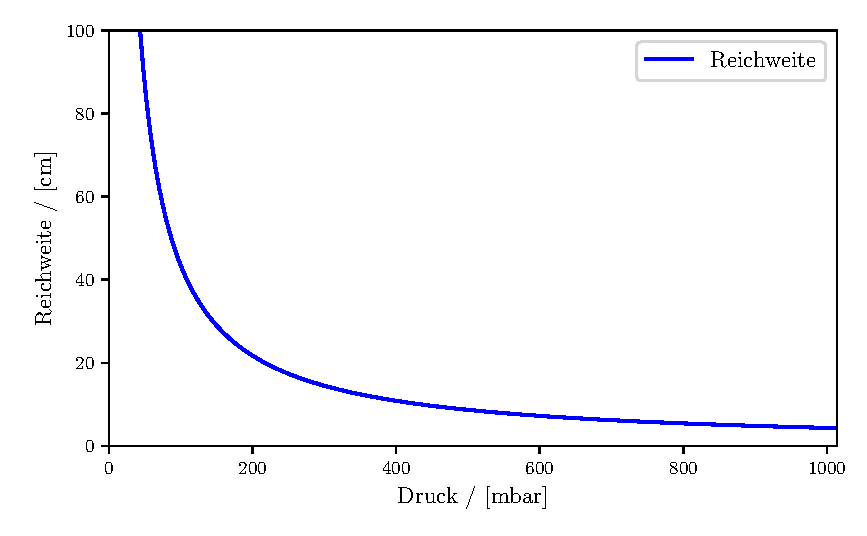
\includegraphics{build/Druck.pdf}
  \caption{Druckabhängige Bethe-Bloch-Formel.}
  \label{fig:Druck1}
\end{figure}

An der Abbildung ist zu erkennen, dass ab etwa einem Druck von $\SI{100}{\milli\bar}$ die Teilchen nur noch minimal in ihrer Reichweite beschränkt werden.
\newpage
\section{Auswertung}
\label{sec:Auswertung}
Sämtliche im Folgenden durchgeführten Ausgleichsrechnungen werden mit der \emph{curve fit} Funktion aus dem für \emph{Python} geschriebenen package \emph{NumPy}\cite{scipy} durchgeführt. Fehlerrechnungen werden mit dem für \emph{Python} geschriebenen package \emph{Uncertainties}\cite{uncertainties} ausgeführt.

\subsection{Verstärkung durch den Amplifier}
Die Pulshöhe des gemessenen Signals des Surface-Barrier-Detektors ist in Abbildung \ref{fig:ohne} zunächst ohne Verstärkung und in Abbildung \ref{fig:mit} mit Verstärkung durch eine Amplifier dargestellt. 
\begin{figure}[H]
\centering
\begin{subfigure}{.5\textwidth}
	\centering
	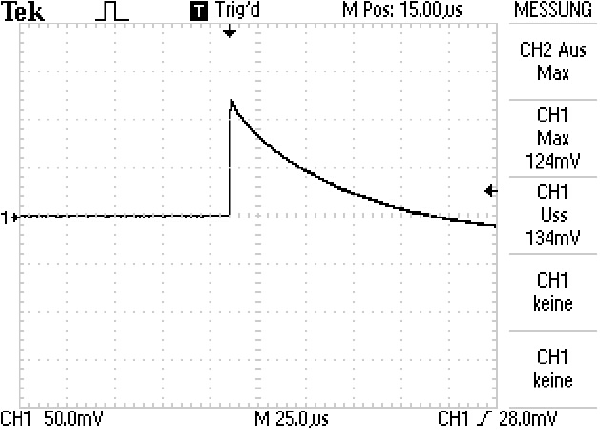
\includegraphics[width=0.95\textwidth]{ressources/ohne.png}
	\caption{Ohne Vorverstärkung}
	\label{fig:ohne}
\end{subfigure}%
\begin{subfigure}{.5\textwidth}
	\centering
	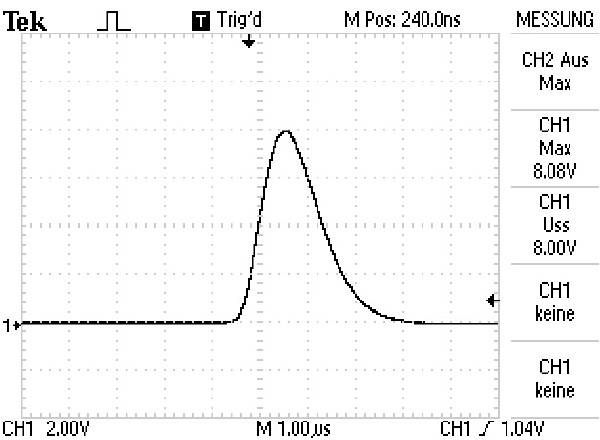
\includegraphics[width=0.95\textwidth]{ressources/mit.png}
	\caption{Nach Vorverstärkung}
	\label{fig:mit}
\end{subfigure}
\caption{Messsignal vor und nach der Verstärkung.}
\label{fig:calib}
\end{figure}

Die aus den Abbildungen entnommenen Impulshöhen und Anstiegszeiten sind im Folgenden aufgelistet: 
\begin{align}
	U_\text{ohne}&=\SI{120}{\milli\volt}\\
	U_\text{mit}&=\SI{8}{\volt}\\
	\\
	t_\text{ohne}&=\SI{1}{\micro\second}\\
	t_\text{mit}&=\SI{1}{\micro\second}
\end{align}
Da diese Werte nur abgelesen worden sind, sind sie als Richtwert anstatt als Messergebisse zu interpretieren. Jedoch kann abgeschätzt werden, dass der Amplifier eine Verstärkung der Spannung um Faktor $68$ verursacht. Im Gegensatz dazu bleibt die Anstiegszeit unverändert. 

\subsection{Aktivität}
Zunächst wird die Aktivität der $\ce{^{241}_{95}Am}$-Probe bestimmt. Hierfür wird der Winkel $\theta=\SI{0}{\degree}$ eingestellt und die Folie entfernt. Bei angelegtem Vakuum werden  $5608$ Counts in einem Zeitraum von $\Delta t= \SI{300}{\second}$ detektiert. Daraus ergibt sich eine Aktivität von $A_{\ce{^{241}_{95}Am}}=\SI{18.7}{\becquerel}
$\\
In der Versuchsanleitung \cite{skript} ist eine Aktivität von $A=\SI{330}{\kilo\becquerel}$ für den Oktober 1994 angegeben. Mit der Halbwertszeit $T_{1/2}=432.2\:$Jahren ergibt sich mit der bis zum Versuchstag vergangenen Zeit $t$ eine aktuelle Aktivität von
\begin{align}
	A_{02.2018}=A_{10.1994}\cdot e^{-\lambda\cdot t}=\SI{317.5}{\kilo\becquerel}
\:.
\end{align}
Dieser Wert bezieht sich dabei auf die komplett Kugeloberfläche mit dem Radius $r=\SI{10.1}{\centi\meter}$. Skaliert auf die Blendenfläche besteht eine theoretische Aktivität von $A_{\text{skaliert}}=\SI{5.0}{\becquerel}
$.


\subsection{Foliendicke}
\label{sec:foliendicke}
In diesem Kapitel soll die verwendete Foliendicke bestimmt werden. Hierzu ist die Pulshöhe in Abhängigkeit des Drucks mit und ohne Folie vermessen worden. Die resultierenden Messwerte sind in Tabelle \ref{tab:ohne_folie} und \ref{tab:mit_folie} dargestellt.
\begin{table}
\centering
\begin{tabular}{c|c|c|c}
Druck in mbar  & $\text{U}_{\text{max}}$ in V & $\text{U}_{\text{min}}$ in V & $\text{U}$ in V\\
\hline
0.026 & 5.00 & 3.52 & 4.26 \pm 0.74\\
20.2 & 4.64 & 3.44 & 4.04 \pm 0.59\\
41.0 & 4.40 & 3.16 & 3.78 \pm 0.62\\
60.2 & 4.32 & 2.72 & 3.52 \pm 0.80\\
86.1 & 4.00 & 2.52 & 3.62 \pm 0.74\\
101.0 & 3.88 & 2.40 & 3.14 \pm 0.71\\
123.4 & 3.64 & 2.16 & 2.90 \pm 0.74\\
141.7 & 3.28 & 1.80 & 2.54 \pm 0.73\\
167.0 & 2.92 & 1.48 & 2.20 \pm 0.72\\
178.5 & 2.80 & 1.44 & 2.12 \pm 0.68\\
203.0 & 2.48 & 1.12 & 1.80 \pm 0.68\\
235.0 & 1.80 & 0.88 & 1.34 \pm 0.46\\
265.0 & 1.30 & 0.68 & 0.99 \pm 0.34\\
\hline
\end{tabular}
\caption{Messwerte der Pulshöhe U bei verschiedenen Drücken ohne Folie}
\label{tab:ohne_folie}
\end{table}

\begin{table}
\centering
\begin{tabular}{c|c|c|c}
Druck in mbar  & $\text{U}_{\text{max}}$ in V & $\text{U}_{\text{min}}$ in V & $\text{U}$ in V\\
\hline
0.026 & 4.32 & 2.12 & 3.22 \pm 1.10\\
19.5 & 3.88 & 1.76 & 2.82 \pm 1.06\\
39.0 & 3.60 & 1.72 & 2.66 \pm 0.94\\
60.3 & 3.32 & 1.24 & 2.28 \pm 1.04\\ 
79.5 & 3.32 & 0.88 & 2.10 \pm 1.22\\
99.5 & 2.60 & 0.88 & 1.74 \pm 0.86\\
123.4 & 2.48 & 0.88 & 1.68 \pm 0.79\\
142.0 & 2.16 & 0.68 & 1.42 \pm 0.74\\
162.6 & 1.72 & 0.68 & 1.20 \pm 0.52\\
182.2 & 1.72 & 0.68 & 1.20 \pm 0.52\\
203.0 & 0.96 & 0.00 & 0.48 \pm 0.48\\
\hline
\end{tabular}
\caption{Messwerte der Pulshöhe U bei verschiedenen Drücken mit $\SI{2}{\micro\meter}$ Goldfolie.}
\label{tab:mit_folie}
\end{table}

Um eine Aussage über die mittlere Pulshöhe treffen zu können, wird für jeden Druck der Mittelwert aus der minimalen und der maximalen Pulshöhe berechnet. In Abbildung \ref{fig:Druck} ist der Puls in Abhängigkeit des Druck dargestellt. Mit einer Ausgleichsrechnung der Form 
\begin{align}
	U(p)=a\cdot p + b
\end{align}
ergeben sich die folgenden Parameter:

\begin{align}
  a_{\text{ohne Folie}} &= \SI{-0.0124+-0.0002}{\volt\per\milli\bar}
 \\
  a_{\text{mit Folie}} &= \SI{-0.0119+-0.0007}{\volt\per\milli\bar}
 \\
  b_{\text{ohne Folie}} &= \SI{4.31+-0.03}{\volt}
 \\
  b_{\text{mit Folie}} &= \SI{3.09+-0.08}{\volt}
.
\end{align}


\begin{figure}
  \centering
  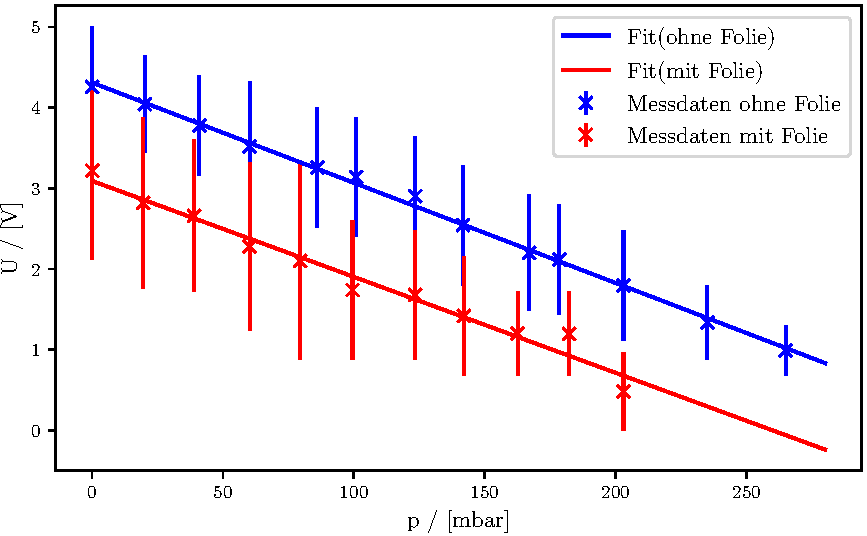
\includegraphics{build/test.pdf}
  \caption{Gemessene Pulshöhe in Abhängigkeit des Druckes mit und ohne
Folie, sowie Ausgleichsgeraden.}
  \label{fig:Druck}
\end{figure}

Zur Bestimmung der Foliendicke wird die Bethe-Bloch-Gleichung \label{bethe} verwendet. Die Dicke der Folie entspricht der Strecke $\Delta x$ und der Energieverlust
\begin{align}
	\Delta E = E_\alpha(1-\frac{b_\text{Folie}}{b_\text{ohne Folie}})
\end{align}
der Differenz der Offsetspannungen. Die Geschwindigkeit wird aus der mittleren Energie wie folgt entnommen:
\begin{align}
	\bar{v}=\sqrt{\frac{E_\alpha(1+\frac{b_{\text{mit}}}{b_{\text{ohne}}})}{m_0}} \:.
\end{align}

Mit den für Gold spezifischen Parametern nach \cite{lenntech} und \cite{pdg}
\begin{align*}
	N_\text{Gold}&=\SI{5.9e28}{\per\meter\squared}\\
	Z_\text{Gold}&=79\; \text{und}\\
	I_\text{Gold}&=\SI{790}{\electronvolt}
\end{align*}
ergibt sich somit eine Foliendicke von $d_{\text{Folie}} = \SI{3.5+-0.2}{\micro\meter}
$.

\subsection{Differentieller Wirkungsquerschnitt}
In Tabelle \ref{tab:Winkel} sind die detektierten Counts in Abhängigkeit des Winkels $\theta$ unter Verwendung einer $\SI{2}{\micro\meter}$ Goldfolie aufgelistet. 


% \begin{table}
% \centering
% \begin{tabular}{c|c|c}
% Winkel in $\si{\degree}$  & $\text{Counts}$ & $\Delta\text{t}$ in s\\
% \hline
% 0 & 3458 & 300 11.526666666666667+/-0.19601587237318877\\
% 0.5 & 3505 & 300 11.683333333333334+/-0.19734346820820914\\
% 1 & 3582 & 300 11.94+/-0.19949937343260005\\
% 1.5 & 3523 & 300 11.743333333333334+/-0.197849550023356\\
% 2 & 3339 & 300  11.13+/-0.19261360284258222\\
% 2.5 & 3150 & 300  10.5+/-0.18708286933869708\\
% 3 & 2857 & 300
% 3.5 & 2624 & 300
% 4.1 & 2459 & 300 
% 4.5 & 2186 & 300 
% 5 & 1902 & 300 
% 6 & 1409 & 300 
% 7 & 968 & 300\\
% 8 & 1057 & 450\\
% 9.1 & 617 & 450\\
% 11.1 & 337 & 600\\
% 13.9 & 133 & 600\\
% 16.8 & 48 & 600\\
% 20 & 33 & 600\\
% \hline
% \end{tabular}
% \caption{Messung der Counts unter verschieden Winkeln mit einer $\SI{2}{\micro\meter}$ Goldfolie.}
% \label{tab:Winkel}
% \end{table}

\begin{table}
    \centering
    \caption{Messdaten.}
    \label{tab:Winkel}
    \sisetup{parse-numbers=false}
    \begin{tabular}{
	S[table-format=2.1]
	S[table-format=2.2]
	@{${}\pm{}$}
	S[table-format=1.2, table-number-alignment = left]
	S[table-format=3.1]
	S[table-format=1.3]
	@{${}\pm{}$}
	S[table-format=1.3, table-number-alignment = left]
	}
	\toprule
	{$Winkel \:/\: \si{\degree}$}		& \multicolumn{2}{c}{$Counts$}		& 
	{$\Delta t \:/\: \si{\second}$}		& \multicolumn{2}{c}{$\sigma \:/\: 10^{-22} \si{\meter\squared}$}		\\ 
	\midrule
    0.0  & 11.5 & 0.2  & 300.0 & 5.32  & 0.09  \\
0.5  & 11.7 & 0.2  & 300.0 & 5.40  & 0.09  \\
1.0  & 11.9 & 0.2  & 300.0 & 5.52  & 0.09  \\
1.5  & 11.7 & 0.2  & 300.0 & 5.42  & 0.09  \\
2.0  & 11.1 & 0.2  & 300.0 & 5.14  & 0.09  \\
2.5  & 10.5 & 0.2  & 300.0 & 4.85  & 0.09  \\
3.0  & 9.5  & 0.2  & 300.0 & 4.40  & 0.08  \\
3.5  & 8.7  & 0.2  & 300.0 & 4.04  & 0.08  \\
4.1  & 8.2  & 0.2  & 300.0 & 3.79  & 0.08  \\
4.5  & 7.3  & 0.2  & 300.0 & 3.37  & 0.07  \\
5.0  & 6.3  & 0.1  & 300.0 & 2.93  & 0.07  \\
6.0  & 4.7  & 0.1  & 300.0 & 2.17  & 0.06  \\
7.0  & 3.2  & 0.1  & 300.0 & 1.49  & 0.05  \\
8.0  & 2.35 & 0.07 & 450.0 & 1.08  & 0.03  \\
9.1  & 1.37 & 0.06 & 450.0 & 0.63  & 0.03  \\
11.1 & 0.56 & 0.03 & 600.0 & 0.26  & 0.01  \\
13.9 & 0.22 & 0.02 & 600.0 & 0.102 & 0.009 \\
16.8 & 0.08 & 0.01 & 600.0 & 0.037 & 0.005 \\
20.0 & 0.06 & 0.01 & 600.0 & 0.025 & 0.004 \\

    \bottomrule
    \end{tabular}
    \end{table}






Zunächst wird der Wirkungsquerschnitt 
\begin{align}
	\sigma=\frac{N_\text{Counts}F}{A_{\ce{^{241}_{95}Am}}N_T}
\end{align}
nach \cite{wiki} bestimmt. Hierbei beschreibt $N_\text{Counts}$ die Anzahl der gemessenen Counts, $F=\SI{20.0}{\milli\meter\squared}
$ die getroffene Detektorfläche, $A_{\ce{^{241}_{95}Am}}$ die Aktivität der $\ce{^{241}_{95}Am}$-Probe und $N_T=2.36 \cdot 10^{18}$ die Anzahl der Goldatome die sich im getroffenen Folienvolumen befinden. Zusätzlich wird mit der Oosterom-und-Strackee-Formel
\begin{align}
	\Omega = 4 \arctan{\left(\frac{x\cdot y}{2z\cdot \sqrt{4z^2+x^2+y^2}}\right)}
\end{align}
der durch die Folie eingenommene Raumwinkel bestimmt. Dabei bezeichnen $x= \SI{2.0}{\milli\meter}
$ und $y= \SI{10.0}{\milli\meter}
$ die Abmessungen der verwendeten Blende und $z= \SI{45.0}{\milli\meter}
$ den Abstand von der Blende bis zur Folie. Somit ergibt sich ein Raumwinkel von $\Omega = \SI{0.01}{\steradian}
$. Anschließend wird der Wirkungsquerschnitt durch den Raumwinkel geteilt und in Abbildung \ref{fig:Wirkungsquerschnitt1} dargestellt. Zusätzlich ist der theoretische Wirkungsquerschnitt, bestimmt durch Gleichung \ref{wq}, eingezeichnet.

\begin{figure}
  \centering
  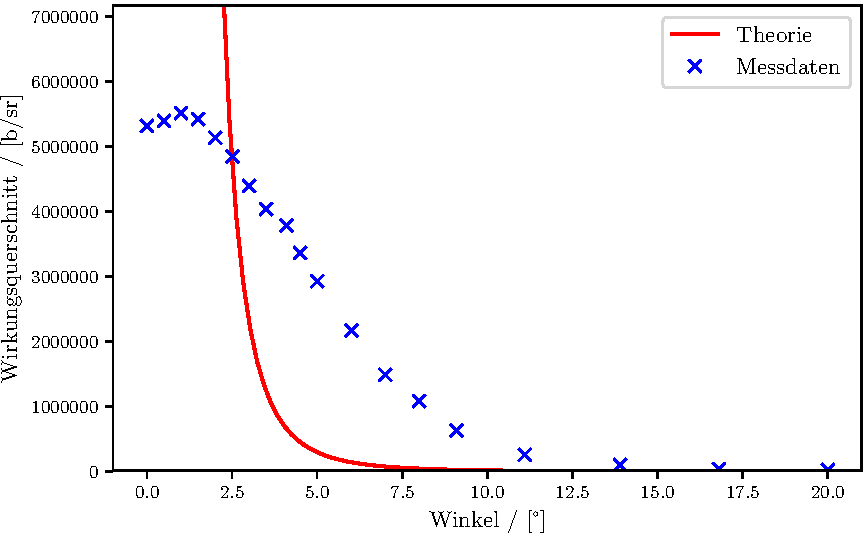
\includegraphics{build/Wirkungsquerschnitt.pdf}
  \caption{Experimenteller und theoretischer Wirkungsquerschnitt in Abhängigkeit des Winkels.}
  \label{fig:Wirkungsquerschnitt1}
\end{figure}


\subsection{Mehrfachstreuuung}
\label{sec:Mehrfachstreuung}
Zur Untersuchung der Mehrfachstreuung sind für die Foliendicken $\SI{2}{\micro\meter}$ und $\SI{4}{\micro\meter}$ bei einem festen Winkel von $\theta=\SI{5}{\degree}$ die detektierten Counts gemessen worden. Die Messwerte sowie der differenzielle Wirkungsquerschnitt sind in Tabelle \ref{tab:divers} aufgelistet.

% \begin{table}
% \centering
% \begin{tabular}{c|c|c}
% Foliendicke in $\si{\micro\meter}$  & $\text{Counts}$ & $\Delta\text{t}$ in s\\
% \hline
% 2 & 1902 & 300\\
% 4 & 1277 & 300\\
% \hline
% \end{tabular}
% \caption{Messung der Counts unter einem $\SI{5}{\degree}$ Winkel für zwei verschiedene Foliendicken des gleichen Materials.}
% \label{tab:divers}
% \end{table}

\begin{table}
    \centering
    \caption{Messung der Counts für zwei verschiedene Foliendicken des gleichen Materials}
    \label{tab:divers}
    \sisetup{parse-numbers=false}
    \begin{tabular}{
	S[table-format=1.1]
	S[table-format=1.1]
	@{${}\pm{}$}
	S[table-format=1.1, table-number-alignment = left]
	S[table-format=3.1]
	S[table-format=1.2]
	@{${}\pm{}$}
	S[table-format=1.2, table-number-alignment = left]
	}
	\toprule
	{$\text{Foliendicke} \:/\: \si{\micro\meter}$}		& \multicolumn{2}{c}{$\text{Counts}$}		& 
	{$\Delta t \:/\: \si{\second}$}		& \multicolumn{2}{c}{$\sigma \:/\: 10^{-22} \si{\meter\squared}$}		\\ 
	\midrule
    2.0 & 6.3 & 0.1 & 300.0 & 2.93 & 0.07 \\
4.0 & 4.3 & 0.1 & 300.0 & 0.98 & 0.03 \\

    \bottomrule
    \end{tabular}
    \end{table}


\subsection{Ordnungzahl-Abhängigkeit}
Als letztes wird in diesem Kapitel die Z-Abhängigkeit der Rutherfordschen Streuformel \ref{wq} nachgewiesen. Hierzu sind die Counts für drei verschiedenen Materialien mit unterschiedlichen Foliendicken, bei einem Winkel von $\theta=\SI{10}{\degree}$ vermessen worden. Die Messergebnisse sind in Tabelle \ref{tab:ordnungszahl} aufgelistet. 

\begin{table}
\centering
\begin{tabular}{c|c|c}
Ordnungszahl & Zählrate in $\si{\per\second}$ & Dicke in $\si{\micro\meter}$\\
\hline
79 & 2.85 \pm 0.03 & 2\\
83 & 0.35 \pm 0.05 & 1\\
13 & 0.68 \pm 0.06 & 3\\
\hline
\end{tabular}
\caption{Gemessene Counts verschiedener Materialien bei einem Winkel von $\SI{10}{\degree}$}
\label{tab:ordnungszahl}
\end{table}


Die Intensität 
\begin{align}
	I=\frac{N_\text{Counts}}{n\cdot d}
\end{align}
wird für die folgende Darstellung auf die Foliendicke $d$ und die Anzahl $n$, der in der Folie enthaltenen Atome, normiert. Mit den Konstanten in Tabelle \ref{tab:Konstanten} wird die jeweilige Anzahl der Atome mit der Gleichung

\begin{align}
	n=\frac{\rho \cdot F \cdot d}{M}\;
\end{align}
bestimmt, dabei beschreibt $\rho$ die Dichte des Materials, $F$ die Fläche der Blende, $d$ die Dicke der Folie und $M$ die atomare Masse des Materials.

\begin{table}
\centering
\begin{tabular}{c|c|c|c}
Material & Dichte in $\si{\gram\per\cubic\centi\meter}$ & Dicke in $\si{\micro\meter}$ & Atommasse in u\\
\hline
Gold & 19.3 & 2 & 196.97\\
Bismut &  9.78 & 1 & 208.98\\
Gold & 2.7 & 3 & 26.98\\
\hline
\end{tabular}
\caption{Verwendete Konstanten für die verschiedenen Materialien.}
\label{tab:Konstanten}
\end{table}

In Abbildung \ref{fig:Wirkungsquerschnitt} ist abschließend die normierte Intensität gegen die Ordnungszahl $Z$ aufgetragen. Zusätzlich, zur Verdeutlichung des mathematischen Zusammenhangs, ist eine lineare Ausgleichsrechnung eingezeichnet.

\begin{figure}
  \centering
  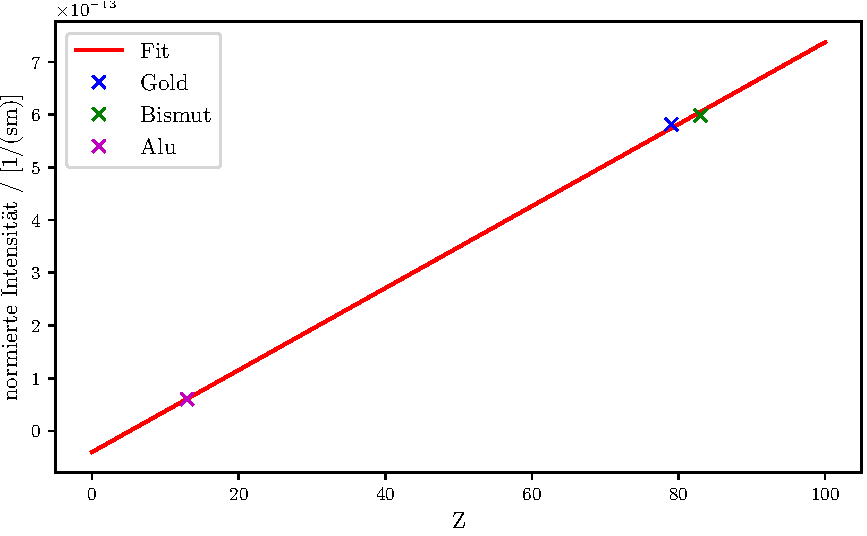
\includegraphics{build/Z.pdf}
  \caption{Nomierte Intensität in Abhängigkeit der Ordnungszahl mit zusätzlicher linearer Ausgleichsrechnung.}
  \label{fig:Wirkungsquerschnitt}
\end{figure}

%%%%%%%%%%%%%%%%%%%%%%%%%%%%%%%%%%%%%%%%%%%%%%%%%%%%%%%%%%%%%%%%%%%%%%%%%%%%%%%%%%%%%%%%%%%%%%%%%%%%%%%%%%%%%%%%%%%%%%%%%%%%%%%%%%%%%%%%%%%%%%%%%%%%%%%%%%%

% % Examples
% \begin{equation}
%   U(t) = a \sin(b t + c) + d
% \end{equation}
%
% \begin{align}
%   a &= \input{build/a.tex} \\
%   b &= \input{build/b.tex} \\
%   c &= \input{build/c.tex} \\
%   d &= \input{build/d.tex} .
% \end{align}
% Die Messdaten und das Ergebnis des Fits sind in Abbildung~\ref{fig:plot} geplottet.
%
% %Tabelle mit Messdaten
% \begin{table}
%   \centering
%   \caption{Messdaten.}
%   \label{tab:data}
%   \sisetup{parse-numbers=false}
%   \begin{tabular}{
% % format 1.3 bedeutet eine Stelle vorm Komma, 3 danach
%     S[table-format=1.3]
%     S[table-format=-1.2]
%     @{${}\pm{}$}
%     S[table-format=1.2]
%     @{\hspace*{3em}\hspace*{\tabcolsep}}
%     S[table-format=1.3]
%     S[table-format=-1.2]
%     @{${}\pm{}$}
%     S[table-format=1.2]
%   }
%     \toprule
%     {$t \:/\: \si{\milli\second}$} & \multicolumn{2}{c}{$U \:/\: \si{\kilo\volt}$\hspace*{3em}} &
%     {$t \:/\: \si{\milli\second}$} & \multicolumn{2}{c}{$U \:/\: \si{\kilo\volt}$} \\
%     \midrule
%     \input{build/table.tex}
%     \bottomrule
%   \end{tabular}
% \end{table}
%
% % Standard Plot
% \begin{figure}
%   \centering
%   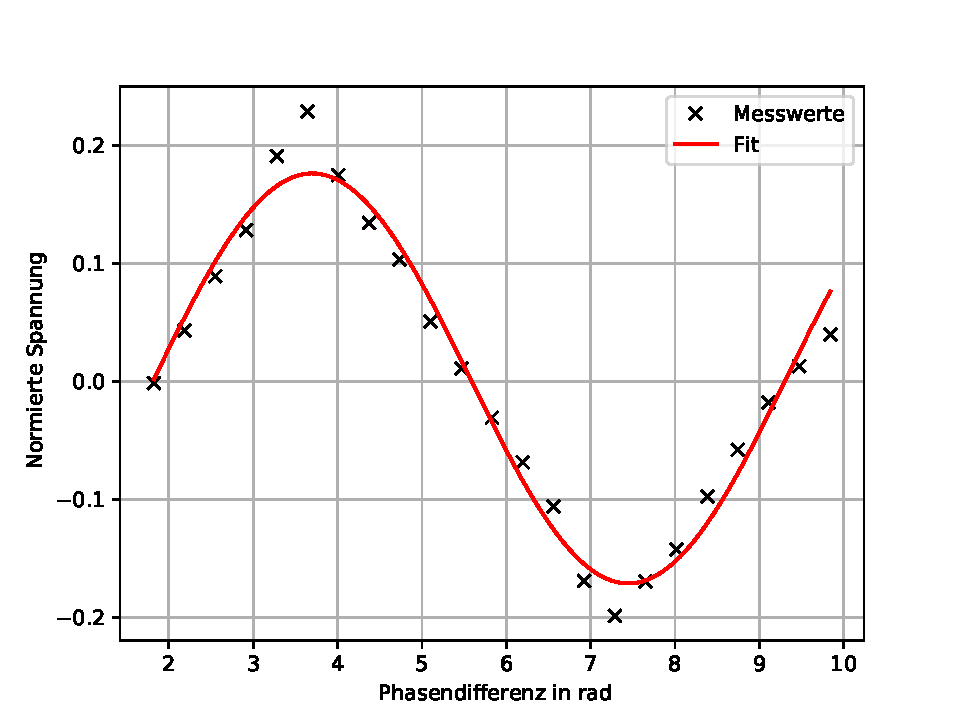
\includegraphics{build/plot.pdf}
%   \caption{Messdaten und Fitergebnis.}
%   \label{fig:plot}
% \end{figure}
%
% 2x2 Plot
% \begin{figure*}
%     \centering
%     \begin{subfigure}[b]{0.475\textwidth}
%         \centering
%         \includegraphics[width=\textwidth]{Abbildungen/Schaltung1.pdf}
%         \caption[]%
%         {{\small Schaltung 1.}}
%         \label{fig:Schaltung1}
%     \end{subfigure}
%     \hfill
%     \begin{subfigure}[b]{0.475\textwidth}
%         \centering
%         \includegraphics[width=\textwidth]{Abbildungen/Schaltung2.pdf}
%         \caption[]%
%         {{\small Schaltung 2.}}
%         \label{fig:Schaltung2}
%     \end{subfigure}
%     \vskip\baselineskip
%     \begin{subfigure}[b]{0.475\textwidth}
%         \centering
%         \includegraphics[width=\textwidth]{Abbildungen/Schaltung4.pdf}    % Zahlen vertauscht ... -.-
%         \caption[]%
%         {{\small Schaltung 3.}}
%         \label{fig:Schaltung3}
%     \end{subfigure}
%     \quad
%     \begin{subfigure}[b]{0.475\textwidth}
%         \centering
%         \includegraphics[width=\textwidth]{Abbildungen/Schaltung3.pdf}
%         \caption[]%
%         {{\small Schaltung 4.}}
%         \label{fig:Schaltung4}
%     \end{subfigure}
%     \caption[]
%     {Ersatzschaltbilder der verschiedenen Teilaufgaben.}
%     \label{fig:Schaltungen}
% \end{figure*}
